\chapter{Curvature as regularization}
\label{chapter:curvature-prior}

The curvature is a geometric property of curves and it measures the rate of change in curve orientation. A straight line has zero curvature while the curvature at corner of a square is infinity. The curvature is measured with respect to the arc-length parametrization, and it is invariant to translations, rotations and reflections (rigid transformations).

In imaging, the most widely use of curvature is, perhaps, as a smooth regularization term. That was the case in the Geometric Active Contour and Chan-Vese image segmentation models of~\cref{chapter:variational-methods-in-image-processing}. The curvature action in these models is closed related with the \emph{curve-shortening flow} applied to the image level curves. Additionally, the curvature also appears in the derivation of the TV denoising model.

Beyond the smoothing role, curvature can be used to favor connectivity, suggesting that its use could be valuable in the segmentation of thin and elongated objects, a difficult class to standard segmentation models. In image inpainting, the \emph{elastica curve} revealed to be a suitable model to mimic the amodal completion phenomenon, believed to be the process behind the human vision in the perception of occluded objects. However, elastica minimization is a challenging task, mainly because of its non-convexity and the $4th$ order expression emerging from its Euler-Lagrange equation.

In~\cref{ch4:sec:curvature-curve-shortening-flow,ch4:sec:diffusion-level-curves-motion}, we recall the definition of curvature and point out its role in some earlier imaging models. In~\cref{ch4:sec:elastica-curve} we describe the elastica curve, and the challenges involved in the minimization of the elastica energy. We dedicate~\cref{ch4:sec:discrete-methods-squared-curvature} to describe discrete models aiming the minimization of the elastica energy, which is an important topic of this thesis.



\section{Curvature and the curve-shortening flow}
\label{ch4:sec:curvature-curve-shortening-flow}

The curvature is a fundamental geometric property of curves and it widely present in geometric imaging models. In this section we start by recalling the curvature definition and some of its mathematical representations. Next we describe the \emph{curve-shortening flow} for planar curves, the one dimensional case of the mean curvature flow.

\subsubsection{Definitions}
In the remain of this section, we assume that every curve is regular, planar and counter-clockwise oriented. Let $C:[0,L(C)]\rightarrow \mathbb{R}^2$ a curve parameterized by arc-length, i.e.,

\begin{align*}
	C(s) &= (x(s),y(s)).
\end{align*}

Let $T(s)$ and $N(s)$ two orthonormal vectors to $C(s)$, i.e., the unitary tangent and normal to $C(s)$. Writing $C(s)$ using these orthonormal vectors we obtain

\begin{align*}
	C(s) &= \left( C(s) \cdot T(s) \right)T(s) + \left( C(s) \cdot N(s) \right)N(s)
\end{align*}

Notice that $\frac{\partial C}{\partial s} = T(s)$, therefore

\begin{align*}
	\frac{\partial C}{\partial s} \cdot \frac{\partial C}{\partial s} = \bignorm{ \frac{ \partial C}{\partial s} }^2 = 1.
\end{align*}

Derivating the last expression in both sides we obtain

\begin{align*}
	0 &= 2\frac{\partial ^2 C}{\partial s} \cdot \frac{\partial C}{\partial s} \\
	  &= 2\frac{\partial ^2 C}{\partial s} \cdot T(s).
\end{align*}

We conclude that $\frac{\partial ^2 C}{\partial s}$ is orthogonal to $T(s)$, and that the curvature is given by the normal component of $\frac{\partial ^2 C}{\partial s}$, i.e.,

\begin{align*}
	\frac{\partial ^2 C}{\partial s} &= \kappa(s) N(s).
\end{align*}

We have several formulations for curvature, some of them listed below (for a full derivation see the appendix). 

\begin{align*}
\begin{array}{rrl}
	\textbf{Arc-length parameterization:} & \displaystyle \kappa(s) &= \displaystyle \bignorm{ \frac{\partial^2 C}{\partial s^2} }. \\[1.5em]	
	\textbf{Arbitrary parameterization:} & \displaystyle \kappa(u) &= \displaystyle \frac{y'x'' - x'y''}{\left( x'^2 + y'^2 \right)^{3/2}}. \\[1.5em]
	\textbf{Implicit function:} & \displaystyle \kappa(x,y) &= \displaystyle -\frac{f_{xx}^2 - 2f_xf_yf_{xy} + f_{yy}^2}{\norm{\nabla f}^3} \\[1.5em]
	&&= \displaystyle \nabla \cdot \left( \frac{\nabla f}{\norm{\nabla f}} \right).
\end{array}
\end{align*}


\subsubsection{Curve-shortening flow}
\label{ch4:sec:curve-shortening-flow}

Let $ t\geq 0$ and $u \in [0,U]$, for some $U>0$. Next, let the $C^{(0)}:[0,U] \rightarrow \mathbb{R}^2$ and $\mathcal{C}(t,u)$ a family of curves such that

\begin{align}
	\mathcal{C}(0,u) & = C^{(0)}(u) \\
	\frac{\partial \mathcal{C}}{\partial t}(t,u) &= v(t,u) N(t,u),
	\label{ch4:eq:curve-normal-flow}
\end{align}

where $v$ is an arbitrary smooth function. The curve ${C}^{(t)}$ is deformed at each point $p$ by an amount $v$ in the normal direction at $p$. Note that any tangent component is irrelevant to curve deformation. From~\cref{ch4:eq:curve-flow} we compute the first variation of curve length of family $\mathcal{C}$

\begin{align*}
	\frac{\partial }{\partial t}L(t) &= \frac{\partial}{\partial t}\int_{0}^{U}{\norm{ \mathcal{C}_u } du} \\
	&= \int_{0}^{U}{ \frac{ \mathcal{C}_u \cdot \mathcal{C}_{ut} }{\norm{\mathcal{C}_u} } du} \\
	&= \int_{0}^{U}{ T \cdot \left( \mathcal{C}_{t} \right)_u  du}.
\end{align*}

Changing from an arbitrary parameterization $u$ to an arc-length one and recalling that $ds=\norm{ \mathcal{C}_u }  du$

\begin{align*}
	\frac{\partial }{\partial t}L(t) &= \int_{0}^{U}{ T \cdot \left( \mathcal{C}_{t} \right)_s \norm{ \mathcal{C}_u }  du} = \int_{0}^{L(\mathcal{C})}{ T \cdot \left( \mathcal{C}_{t} \right)_s ds}. 	
\end{align*}

Using~\cref{ch4:eq:curve-normal-flow} we obtain

\begin{align*}
	\frac{\partial }{\partial t}L(t) &= \int_{0}^{L(\mathcal{C})}{T \cdot (-\kappa vT + v_sN) ds } = - \int_{0}^{L(\mathcal{C})}{\kappa v ds} = -<\kappa,v>.
\end{align*}

From which we conclude that length decreases the fastest by choosing $v=\kappa$. We define the \emph{curve-shortening flow} (CS flow) of curve $C^{(0)}(u)$ as the family $\mathcal{C}(t,u)$ such that

\begin{align}
	\mathcal{C}(0,u) & = C^{(0)}(u) \\
	\frac{\partial \mathcal{C}}{\partial t}(t,u) &= \kappa(t,u) N(t,u).
	\label{ch4:eq:curve-shortening-flow}
\end{align}


\textbf{Example:} Let $C^{(0)}$ be a circle of radius $R_0$, i.e.,  $C^{(0)} = R_0( \cos t, \sin t)$. From~\cref{ch4:eq:curve-shortening-flow} we conclude that for every $t \geq 0$, $C^{(t)}$ is a circle of radius $R(t)$ where

\begin{align}
	\frac{\partial R}{\partial t} &= -\frac{1}{R}  \rightarrow R(t) = \sqrt{R_0^2 - 2t}.
	\label{ch4:eq:curvature-flow-circle}
\end{align}

Moreover, the curve collapses to a single point in time $t=\frac{R_0^2}{2}$. The curvature flow has many interesting properties~\cite{huisken84flow,gage86heat,ecker08heat}. Among them,

\begin{itemize}
	\item[]{\textbf{Comparison principle:} Let $C_1$,$C_2$ two closed curves such that $C_1^{(0)}$ is in the interior of $C_2^{(0)}$. Then $C_1^{(t)}$ is in the interior of $C_2^{(t)}$ for every $t$.}
	\item[]{\textbf{Convexity preserving:} A convex curve $C^{(0)}$ stays convex for all $t$.}
	\item[]{\textbf{Point collapsing:} Let $C^{(0)}$ a closed curve. There exists a time $t$ in which $C^{(t)}$ describes a circle and it follows~\cref{ch4:eq:curvature-flow-circle} until collapsing into a single point.}
	\item[]{\textbf{Perimeter minimization:} The curvature flow is the continuous deformation that decreases the perimeter of a single closed curve the fastest.}
\end{itemize}


The CS flow appeared in the Chan-Vese and Geometric Active Contour models for image segmentation in~\cref{chapter:variational-methods-in-image-processing} in its level set formulation~\cite{osher88fronts}

\begin{align}
	\frac{\partial f}{\partial t} &= \norm{\nabla f}\nabla \cdot \left( \frac{\nabla f}{\norm{\nabla f}} \right).
	\label{ch4:eq:implicit-curvature-flow}
\end{align}

In this case, each of the image level curves describes a CS flow.

\begin{figure}
\center
\subfloat[]{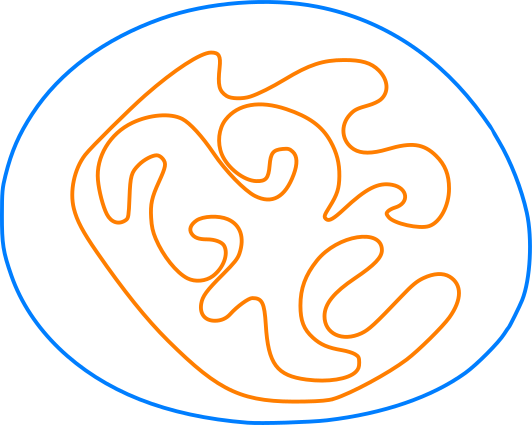
\includegraphics[scale=0.36]{figures/chapter4/curve-shortening-flow/1.png}}\hspace{1em}
\subfloat[]{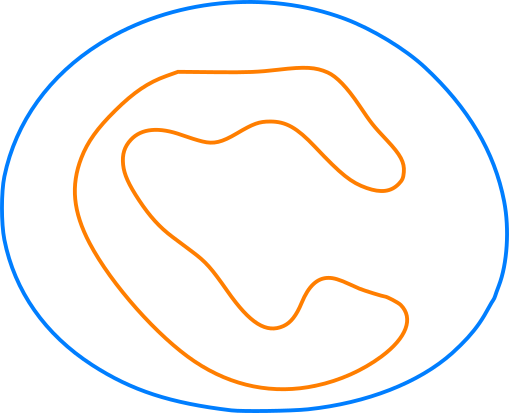
\includegraphics[scale=0.36]{figures/chapter4/curve-shortening-flow/2.png}}\hspace{1em}
\subfloat[]{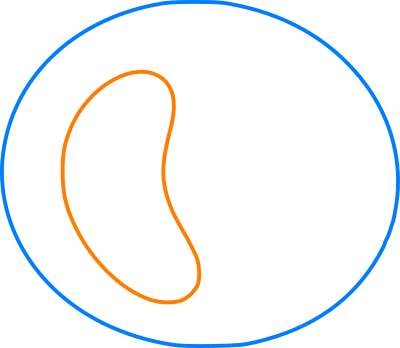
\includegraphics[scale=0.36]{figures/chapter4/curve-shortening-flow/3.png}}\hspace{1em}
\subfloat[]{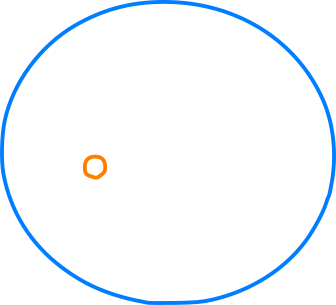
\includegraphics[scale=0.36]{figures/chapter4/curve-shortening-flow/4.png}}
\caption{\textbf{CS flow in action.} CS flow at different times in evolution. In this example we observe the CS flow properties listed in the text.}
\end{figure}



\section{Diffusion and level curves motion}
\label{ch4:sec:diffusion-level-curves-motion}

Several models in~\cref{chapter:variational-methods-in-image-processing} are stated as diffusion processes, but quite often a level curve evolution interpretation is more convenient. In this section we analyze the role of curvature, its properties in earlier models of image processing and how the dual interpretation of these models help us to gain extra insight on them.

\subsubsection{Curvature in denoising and image segmentation}

The necessary optimality condition of the total variation denoising energy is given by

\begin{align}
	\nabla \cdot \left( \frac{\nabla f}{\norm{\nabla f}} \right) + \lambda( f_{\widetilde{\vec{I}}} - f ) &= 0.
	\label{ch4:eq:total-variation-optimal-condition}
\end{align}

The solution of~\cref{ch4:eq:total-variation-optimal-condition} is the steady state of the  anisotropic diffusion

\begin{align}
	u(0,x) &= f(x) 	\label{ch4:eq:tv-flow-1} \\
	\frac{\partial u}{\partial t} &= \nabla \cdot \left( \frac{\nabla f}{\norm{\nabla f}} \right) + \lambda( f_{\widetilde{\vec{I}}} - f ). \label{ch4:eq:tv-flow-2}
\end{align}

Note the similarity between~\cref{ch4:eq:tv-flow-2} and the level set formulation of the CS flow in~\cref{ch4:eq:implicit-curvature-flow}. If $\lambda=0$, we denote~\cref{ch4:eq:tv-flow-1,ch4:eq:tv-flow-2} the \emph{TV flow}\cite{bellettini02total}. Interestingly, both CS flow and TV flow decrease total variation of $f$, but in different ways. The CS flow tends to deform the boundary of objects and decreasing total variation by perimeter minimization. The TV flow, on the other hand, preserves the boundary for longer and it decreases the TV by decreasing the surface height, i.e., the color intensity of the pixels(see~\cref{ch4:fig:minimization-tv-curvature-tv-flow}).

Naturally, the CS flow can also be used to do image denoising. If we think of noise as small artifacts with high gradient of color, the level curves corresponding to noise will have a very small radius, and will collapse faster than other level curves (see~\cref{ch4:fig:denoising-tv-curvature}). 


In the geometric active contours model for image segmentation, the level sets of a predefined function $u$ (e.g., a smoothed version of function $1-\lambda_C$ where $C$ is a set that contains the object to be segmented) describes a CS flow motion modulated by an edge detector function $g$ (e.g., $g=(1+\norm{ \nabla f })^{-1}$).

\begin{align*}
	u(0,x,y) &= u(x,y) \nonumber \\
	\frac{du}{dt} &= g( \norm{\nabla f} )\norm{\nabla u}\nabla \cdot \left( \frac{\nabla u}{\norm{\nabla u}}  + v \right),
\end{align*}



\begin{figure}
\center
	\subfloat{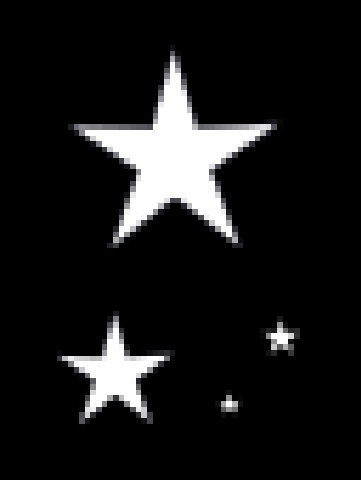
\includegraphics[scale=0.15,valign=t]{figures/chapter4/tv-curvature-stars/curvature/stars.png}}\hspace{0.2em}
	\begin{tabular}[t]{m{0.25cm}cc|cc}
	& \multicolumn{2}{c|}{$\norm{\nabla f_I}=25$} & \multicolumn{2}{c}{$\norm{\nabla f_I}=15$} \\
	\hline
	\rotatebox{90}{CS flow} & \figTable{0.2}{figures/chapter4/tv-curvature-stars/curvature/stars-25.png} & \figTable{0.2}{figures/chapter4/tv-curvature-stars/curvature/levels-stars-25.png} & \figTable{0.2}{figures/chapter4/tv-curvature-stars/curvature/stars-15.png} & \figTable{0.2}{figures/chapter4/tv-curvature-stars/curvature/levels-stars-15.png} \\
	\rotatebox{90}{TV flow} & \figTable{0.2}{figures/chapter4/tv-curvature-stars/tv/stars-25.png} & \figTable{0.2}{figures/chapter4/tv-curvature-stars/tv/levels-stars-25.png} & \figTable{0.2}{figures/chapter4/tv-curvature-stars/tv/stars-15.png} & \figTable{0.2}{figures/chapter4/tv-curvature-stars/tv/levels-stars-15.png}
	\end{tabular}
	\caption{\textbf{Minimizing TV energy with TV flow and CS flow.}Both flows decrease the image total variation, but CS flow tends to deform object boundaries while doing so. On the other hand, TV flow reduces the image contrast.}
	\label{ch4:fig:minimization-tv-curvature-tv-flow}	
\end{figure}

\begin{figure}
\center
\subfloat{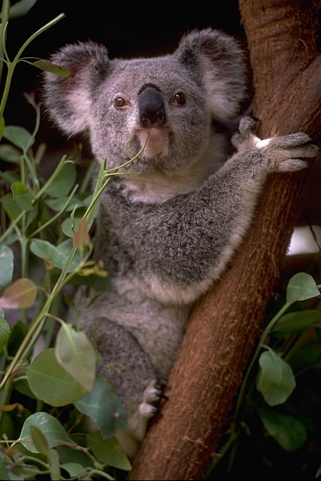
\includegraphics[scale=0.224,valign=t]{figures/chapter4/tv-curvature-coala/curvature/coala-original.png}}\hspace{0.2em}\setcounter{subfigure}{0}
\subfloat[Noisy Image]{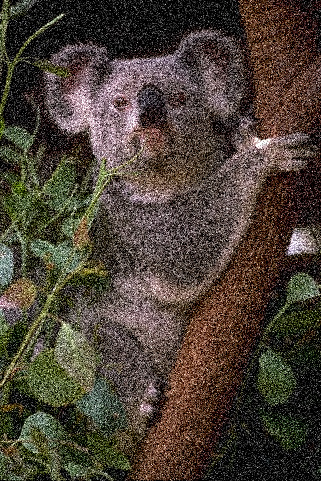
\includegraphics[scale=0.32,valign=t]{figures/chapter4/tv-curvature-coala/curvature/coala-noise.png}}\hspace{1em}
\subfloat[CS flow]{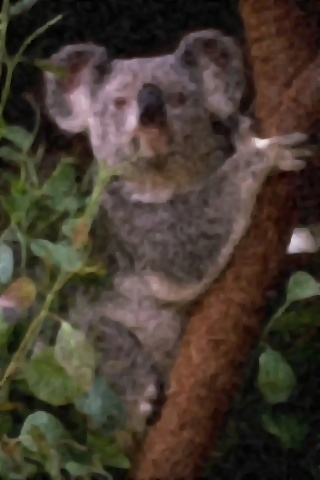
\includegraphics[scale=0.32,valign=t]{figures/chapter4/tv-curvature-coala/curvature/coala-30.png}}\hspace{1em}
\subfloat[TV flow]{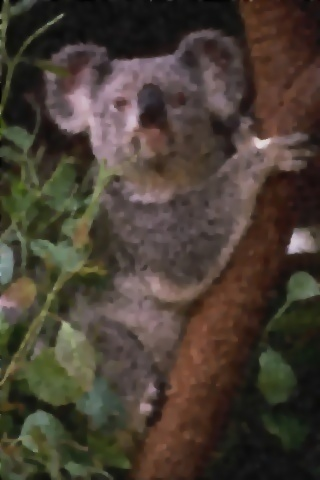
\includegraphics[scale=0.32,valign=t]{figures/chapter4/tv-curvature-coala/tv/coala-30.png}}
\caption{\textbf{TV denoising using CS and TV flow.}Results are quite similar, but TV flow image is sharper, although with lower contrast than CS flow. Images (b) and (c) have the same TV value.}
\label{ch4:fig:denoising-tv-curvature}
\end{figure}

\subsubsection{Curvature and the connectivity principle applied to inpainting}

We recall that the inpainting problem consists into reconstructing a collection of missing patches $\mathcal{P}$ of the image. The earlier inpainting model~\cite{bertalmio00image}  diffuses image information through the patches boundaries. The particularity of this model is that the Laplacian (heat equation) is diffused along the image level lines. Besides its impressive results, this models does not possess an important property which is expected in inpainting models: the \emph{connectivity principle}.


\begin{figure}
\center
\subfloat[Amodal completion.\label{ch4:fig:amodal-completion}]{
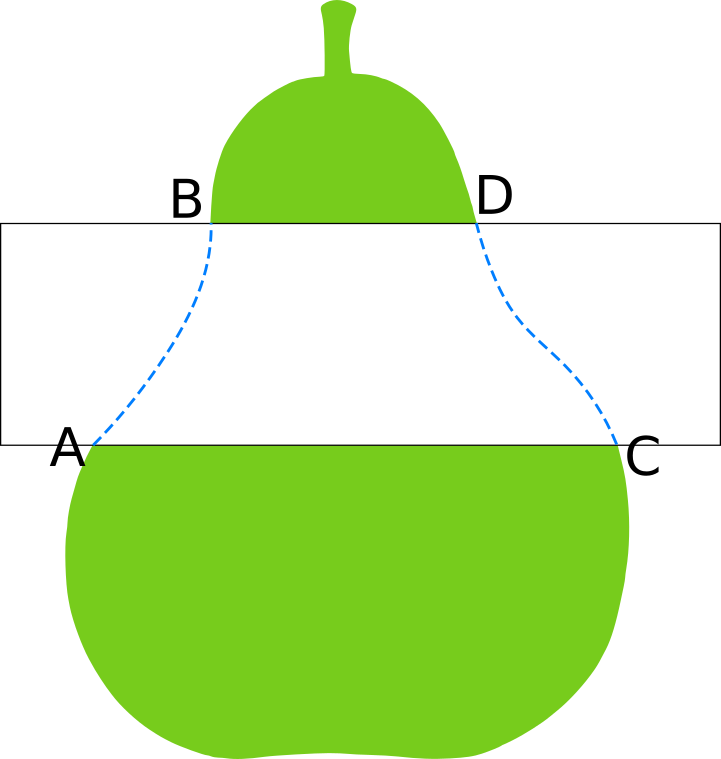
\includegraphics[scale=0.36]{figures/chapter4/amodal-completion.png}
}\hspace{3em}
\subfloat[Thin and elongated object segmentation.\label{ch4:fig:connectivity-principle}]{
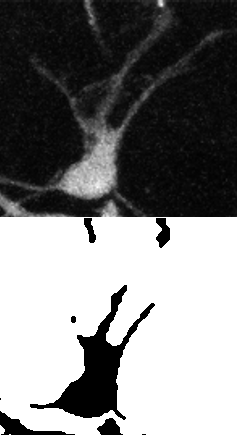
\includegraphics[scale=0.45]{figures/chapter4/vessels-bad-seg.png}
}
\caption{\textbf{Connectivity principle.} In~\cref{ch4:fig:amodal-completion}, an illustration of amodal completion, the process followed by the human vision to complete the boundary of occluded object with curves of low curvature ant that conform the most with the direction of the endpoints. In~\cref{ch4:fig:connectivity-principle} a vessel segmentation with length penalization term only. Curvature favors connected objects.}
\end{figure}

Studies of the Gestalt school of psychology suggest that the human vision, by a process called amodal completion~\cite{mumford94elastica}, completes the boundary of partially occluded object with a short and low curvature curve, as illustrated in~\cref{ch4:fig:amodal-completion}. The model proposed in~\cite{chan01nontexture} is a TV flow modulated by the curvature of the image level curves. 

\begin{align}
	u(0,x,y) &= f(x,y) \nonumber \\
	\frac{\partial u}{\partial t} &= \nabla \cdot \left( |\kappa(t)|\frac{\nabla f}{\norm{f}} \right) .
	\label{ch4:eq:inpainting-curvature-driven-diffusion}
\end{align}

The diffusion in~\cref{ch4:eq:inpainting-curvature-driven-diffusion} is stronger at points of high curvature with respect to its level curves. This model partially achieves the connectivity principle (see~\cref{ch4:fig:inpainting-curvature-driven-diffusion}), but the completion is done only for very small regions. 

The connectivity principle suggests that the curve connecting the endpoints of an occluded object should minimize some energy with respect the curvature. Moreover, the segmentation of thin and elongated objects may also benefit from a curvature term, since classical methods have difficulties to give connected solutions. In the next section we describe the Elastica, the curve that minimizes the squared curvature along its length.

\begin{figure}
\center
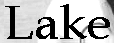
\includegraphics[scale=1]{figures/chapter4/inpainting-cdd/lake-1.png}\hspace{0.5em}
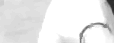
\includegraphics[scale=1]{figures/chapter4/inpainting-cdd/lake-2.png}\hspace{3em}
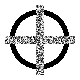
\includegraphics[scale=0.6]{figures/chapter4/inpainting-cdd/circle-1.png}\hspace{0.5em}
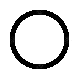
\includegraphics[scale=0.6]{figures/chapter4/inpainting-cdd/circle-2.png}
\caption{\textbf{Inpainting by curvature driven diffusions.}\cite{chan01nontexture} The diffusion process modeled by~\cref{ch4:eq:inpainting-curvature-driven-diffusion} completes the features disconnected by the inpainting mask.}
\label{ch4:fig:inpainting-curvature-driven-diffusion}
\end{figure}



\section{Elastica curve}
\label{ch4:sec:elastica-curve}

In 1691 James Bernoulli pose a challenge to your colleagues: What is the form taken by an elastic beam whose its endpoint $A$ is kept fixed in the ground while a weight is attached to its other endpoint $B$ such that the tangent at each of the endpoints are perpendicular? A simplified scheme is presented in~\cref{ch4:fig:james-scheme-elastica}.

\begin{figure}
\center
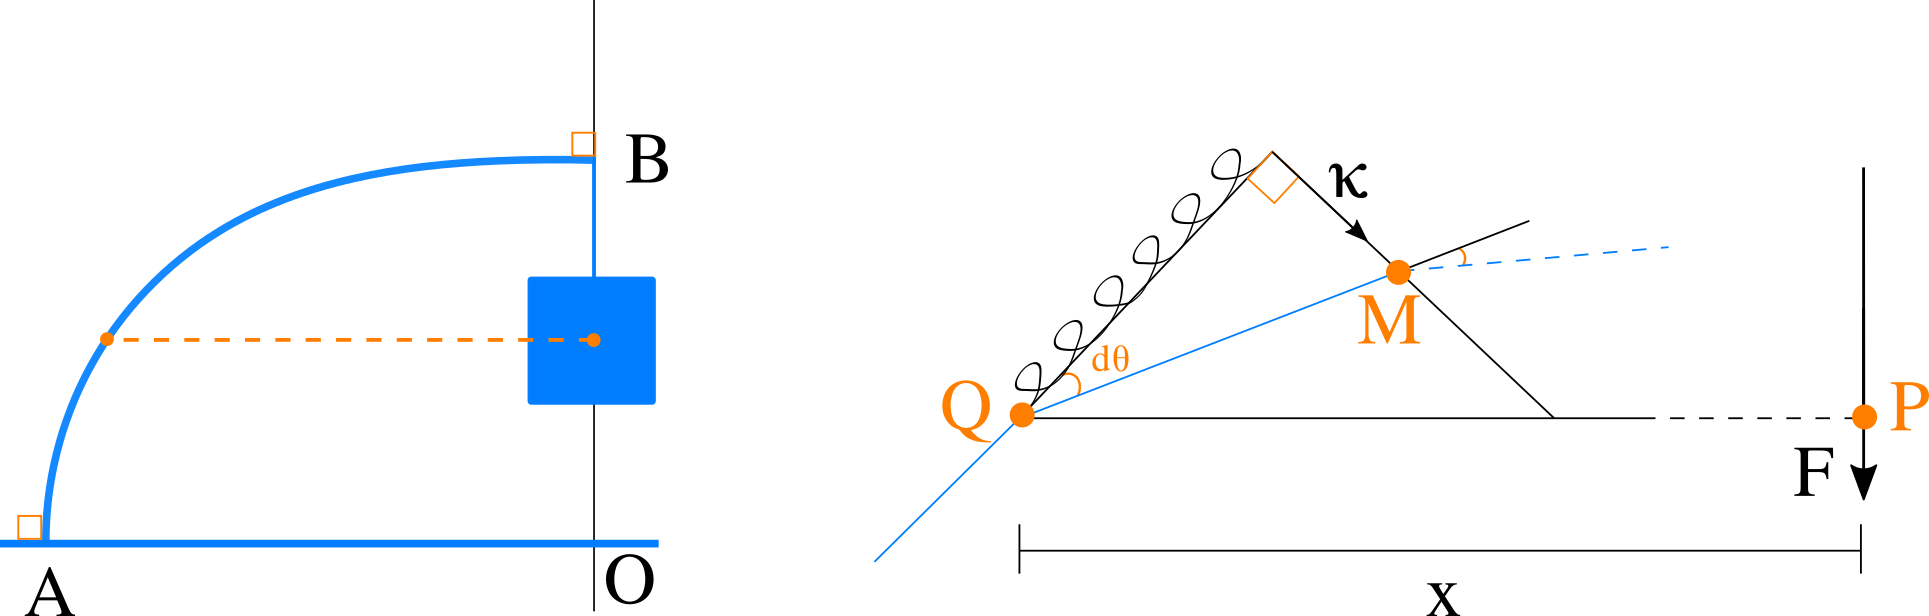
\includegraphics[scale=0.36]{figures/chapter4/elastica/james-scheme.png}
\caption{\textbf{Elastic beam and James Bernoulli's solution.} In equilibrium, the moments at the two ends of the virtual lever $PQM$ should cancel, implying that the curvature is a linear function of $x$ if we assume the spring behaves in accordance with Hooke's law.}
\label{ch4:fig:james-scheme-elastica}
\end{figure}

By using mechanical principles, James concluded that the curvature of such curve at some point $Q$ can be written as a linear function of the distance from $Q$ to the line $BO$, i.e., $\kappa(x) = cx$. One can show that~\cite{levien08elastica,truesdell60rational},

\begin{align}
	\frac{\partial y}{\partial x} &= \frac{cx^2}{ \sqrt{1-c^2x^4} }.
	\label{ch4:eq:rectangular-elastica}
\end{align}

The curve modeled by~\cref{ch4:eq:rectangular-elastica} is called the \emph{rectangular elastica}. The expression in the right cannot be integrated using elementary functions and is a member of the class of elliptic integrals. Fortunately, Euler has shown that one can express not only the rectangular elastica, but its general version in the form of a minimization principle. 

The generalized elastica in $2$D is the planar curve $C$ of fixed length $L$ whose endpoints have known tangents $C'(0)=\theta_0,C'(L)=\theta_L$ and minimizes the energy $\int_{C} \kappa^2 ds$.

\begin{align*}
	\begin{array}{rl}
		\displaystyle \min_{C} \int_{C}{\kappa ^2} \\[1em]
		\text{subject to}& \norm{C} = L,\\
		& C'(0) = \theta_0, \\
		& C'(L) = \theta_L.
	\end{array}	
\end{align*}

Given parameters $\alpha \geq 0, \beta \geq 0$ we incorporate the isoperimetric constraint in the objective function (can be interpreted as a Lagrange multiplier) to define the Elastica energy as

\begin{align}
	E(C) &= \int_{C}{\alpha + \beta \kappa^2 ds}.
	\label{ch4:eq:elastica-energy}
\end{align}

If we do not impose any constraint in~\cref{ch4:eq:elastica-energy}, its minimization is interesting only if $\alpha >0$ and $\beta >0$ and we call this problem the \emph{free Elastica}. On the other hand, if one imposes constraints to the minimization of~\cref{ch4:eq:elastica-energy}(e.g., fixed tangent endpoints), we refer to this problem as the \emph{unconstrained Elastica}.

One can easily derive the solution of the free Elastica for a closed curve. Setting $\beta=0$, the minimization of~\cref{ch4:eq:elastica-energy} behaves as the curve-shortening flow of section~\cref{ch4:sec:curve-shortening-flow}. On the other hand, if we set $\alpha =0$, the minimum is a disk of infinite radius. For the intermediate case, with both parameters greater than zero, it is easy to see that the solution is a circle $C_r$ of some radius $r$, therefore

\begin{align*}
	C_r = \argmin_C E(C) \rightarrow \frac{ \partial}{\partial r} \int_{C_r}{\alpha + \beta \kappa^2 ds} &= 0 \\
	\frac{\partial}{\partial r} \big( \alpha 2\pi r + \beta \pi/r \big) & = 0 \\
	r &= \left(\frac{\beta}{\alpha}\right)^{1/2}.
\end{align*}

In general, a planar curve $C$ minimizing the Elastica energy satisfies the following Euler-Lagrange equation~\cite{chan02elasticainpainting,singer08lectures}

\begin{align}
		2\kappa_{ss} + \kappa^3 = \frac{\alpha}{\beta}\kappa \Leftrightarrow \frac{\partial ^4 C}{\partial s^4} + \frac{\partial ^2 C}{\partial s^2}^3 = \frac{\alpha}{\beta}\frac{\partial ^2 C}{\partial s^2}.
		\label{ch4:eq:euler-lagrange-equation-elastica}
\end{align}


This fourth order expression is the main difficult in minimizing the Elastica. In the following we are going to describe some models that attempt to minimize the Elastica and the strategies employed.

\subsubsection{Imaging models using the Elastica}

In~\cite{chan02elasticainpainting} the authors propose an inpainting model in which the image level lines interrupted by the inpainting domain are completed by Elastica curves. The key is to define an energy that minimize each of the level curves in terms of the Elastica simultaneously. Given an image $f_I:\Omega \rightarrow [0,1]$, let $\Gamma_{\lambda}$ be one of its level curve, i.e.,

\begin{align*}
	\Gamma_{\lambda} &= \left\{ x \; | \; f_I(x)=\lambda \right\}.
\end{align*}

Therefore, we minimize each level curve in terms of the Elastica energy by minimizing the functional

\begin{align}
	\int_{0}^{1}{ \int_{\Gamma_{\lambda}}{ \left( \alpha + \beta \kappa ^2 \right) dsd\lambda}} = \int_{0}^{1}{ \int_{\Gamma_{\lambda}}{ \left(\alpha + \beta \nabla \cdot \left(\frac{\nabla f_I}{\norm{\nabla f_I}}\right) ^2 \right) dsd\lambda}}
	\label{ch4:eq:elastica-all-level-curves}
\end{align}

Next, let $dt$ be the length element in the normal direction of the level curves. Therefore,

\begin{align*}
	\frac{d \lambda}{d t} &= \norm{\nabla f_I} \rightarrow d\lambda = \norm{\nabla f_I}dt.
\end{align*}

Replacing the last expression in~\cref{ch4:eq:elastica-all-level-curves} we obtain

\begin{align}
	\int_{0}^{1}{ \int_{\Gamma_{\lambda}}{ \left(\alpha + \beta \nabla \cdot \left(\frac{\nabla f_I}{\norm{\nabla f_I}}\right) ^2 \right)\norm{\nabla f_I} dsdt}} &= \int_{\Omega}{ \left(\alpha + \beta \nabla \cdot \left(\frac{\nabla f_I}{\norm{\nabla f_I}}\right) ^2 \right)\norm{\nabla f_I}d\Omega}.
	\label{ch4:eq:chan-elastica-inpainting}
\end{align}

The last expression is derived from the fact that $dt$ and $ds$ are orthogonal length elements. The authors propose a finite difference scheme for the gradient flow derived from the Euler-Lagrange of~\cref{ch4:eq:chan-elastica-inpainting}, which happens to be of $4th$ order. The high order poses some issues with numerical instability, namely the definition of the time step and convergence analysis, which is skipped. The running time is also quite high even for small inpainting domains. Moreover, one can expect a local solution at most, and giving the highly non-convex character of the equation, an acceptable local solution might be very difficult to be found without a conveniently chosen initial solution. Finally, the  method tends to produce blurry edges even for small inpainting domains. 

The numerical instability arising from~\cref{ch4:eq:chan-elastica-inpainting} is lessen by the $3rd$ order gradient flow proposed in~\cite{ballester01filling}. The idea is to create a new variable $\theta$ to replace the unstable term $\nabla f_I / \norm{\nabla f_I}$ and include a penalization term that forces $\theta$ to assume the value of its original interpretation. The energy to be minimized is closely related to~\cref{ch4:eq:chan-elastica-inpainting} and is written as

\begin{align}
	\int_{\Omega}{a|\nabla \cdot \theta|^2\left(\alpha + \beta \norm{ k * f_I}\right)d\Omega} + \int_{\Omega}{ \norm{\nabla f_I} - \theta \cdot \nabla f_I d_{\Omega}},\quad \norm{\theta} \leq 1.
	\label{ch4:eq:ballester-inpainting}
\end{align}

The kernel $k$ (e.g. Gaussian) smooths image $f_I$ and is included due to numerical reasons. Nonetheless,~\cref{ch4:eq:ballester-inpainting} suffers from similar issues to those of~\cref{ch4:eq:chan-elastica-inpainting}. Generally, PDE-based methods encounter difficulties in producing solutions with discontinuities, one of the main features of images.

A discrete approach to inpainting is proposed in~\cite{masnou98inpainting}. The model's first step is to identify pairs of admissible T-junctions, i.e., pixels in the outer boundary of the inpainting domain that have the same color value and orientation (see~\cref{ch4:fig:masnou-tjunctions}). Due to a property of level curves, for every value color value $\lambda$ there is an even number of T-junctions. Next, let $J$ be the set of T-junctions and $\Gamma_j^t$ a curve connecting an admissible pair $(j,t)$. Additionaly, we denote $\theta_j,\theta_t$ the respective angles the curve $\Gamma_j^t$ makes with the associated level set at $j$ and $t$. The authors propose to find a matching $\mathcal{M}=\{ (j,t) \; | \; j,t\text{ admissible} \}$ and its respective curves such that it minimizes the energy

\begin{figure}
\center
\subfloat[T-junctions illustration~\cite{ambrosio03direct}\label{ch4:fig:masnou-tjunctions}]{
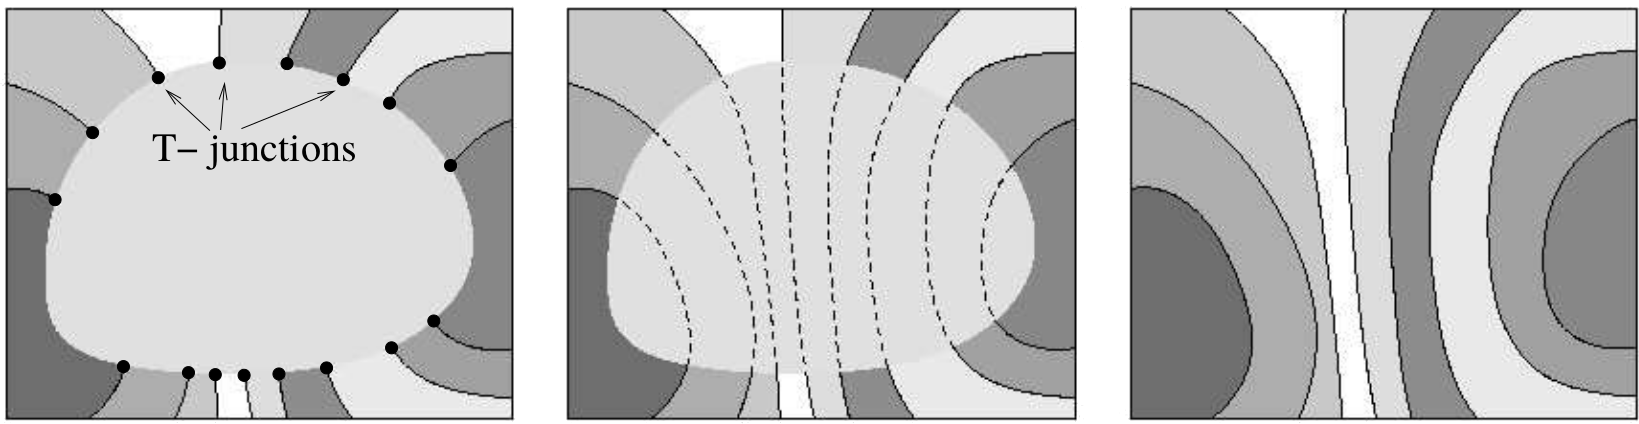
\includegraphics[scale=0.25]{figures/chapter4/masnou/tjunctions.png}}

\subfloat[Inpainting by~\cite{masnou98inpainting}\label{ch4:fig:masnou-inpainting}]{
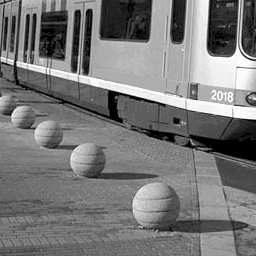
\includegraphics[scale=0.5]{figures/chapter4/masnou/tram-1.png}
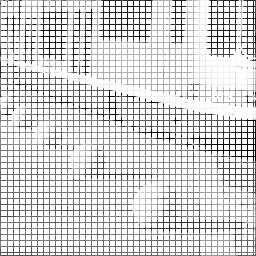
\includegraphics[scale=0.5]{figures/chapter4/masnou/tram-2.png}
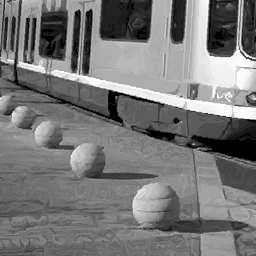
\includegraphics[scale=0.5]{figures/chapter4/masnou/tram-3.png}
}
\caption{\textbf{Discrete inpainting.} In~\cref{ch4:fig:masnou-tjunctions} an illustration of T-junctions and an ideal completion of the level lines; in~\cref{ch4:fig:masnou-inpainting} we have the original image in the left, the image to be inpainted in the middle and the result of the discrete inpainting in the right. }
\end{figure}

\begin{align}
	\sum_{(j,t) \in \mathcal{M}}{ \int_{\Gamma_j^t}{\alpha + \beta |\kappa|ds} + \theta_j + \theta_t }.
	\label{ch4:eq:masnou-inpainting}
\end{align}


Assuming that one knows the optimal matching $\mathcal{M}$, the curves connecting the T-junctions pairs are geodesics. In the plane, that means that the T-junctions are connected by polygonal curves. An ingenious dynamic programming algorithm is conceived  by exploiting the causality relation imposed by the non-crossing constraint of the level curves and excellent results are obtained. In particular, the algorithm can reconstruct large inpainting domains and does not produce blurry edges (see~\cref{ch4:fig:masnou-inpainting}). However,~\cref{ch4:eq:masnou-inpainting} cannot produce curvy level lines.


The work of~\cite{masnou98inpainting} illustrates an advantage of discrete approaches to image models: discontinuities are naturally implemented. To find a discrete model is not a trivial task, and sometimes a compromise needs to be done in order to achieve efficiency, as it was the case in~\cite{masnou98inpainting}, in which the absolute value of the curvature is used instead of its square. In the next section we are going to describe some discrete models for Elastica in its most known form, i.e., using the square of the curvature.


\section{Discrete methods and squared curvature}
\label{ch4:sec:discrete-methods-squared-curvature}

\subsubsection{Discrete elastica}

Let $\mathcal{P}_n=\{p_i \; | \; 1 \leq i \leq n\}$ a sequence of $n$ points describing a polygonal line. We define the following elements (an illustration is given in~\cref{ch4:fig:bruckstein-polygonal-line}).

\[
\begin{array}{rll}
\text{Segment length:} & \quad \ell_i,& \quad 1 \leq i \leq n\\[0.5em]
\text{Segment angle:} & \quad \psi_i,& \quad 1 \leq i \leq n-1\\[0.5em]
\text{Angle deviation:} & \quad \theta_i,& \quad 1 \leq i \leq n-2.
\end{array}
\]

\begin{figure}
\center
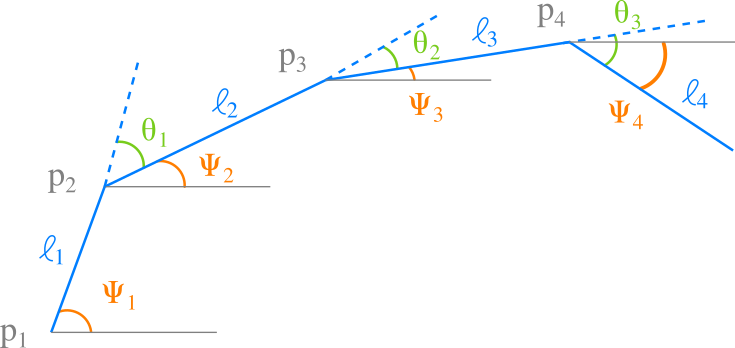
\includegraphics[scale=0.6]{figures/chapter4/bruckstein/polygonal-line.png}
\caption{\textbf{Discrete elastica.} The curvature is approximated by $\theta_i/l_i$.}
\label{ch4:fig:bruckstein-polygonal-line}
\end{figure}

Given parameters $\alpha \geq 0,\beta \geq 0$ and a fixed length segment $\ell$, the discrete elastica~\cite{bruckstein01discrete} is defined as

\begin{align}
	E(\vec{\theta},\ell) &= \ell \cdot \sum_{1 \leq i \leq n-2}{ \alpha + \beta \left(\frac{\theta_i}{\ell}\right)^2} = \sum_{1 \leq i \leq n-2}{ \alpha \ell + \beta \frac{\theta_i^2}{\ell}}.
	\label{ch4:eq:discrete-elastica}
\end{align}

Without loss of generality, we assume that the curve starts at the origin with tangent $\psi_1=t_1$ and ends at point $(L,0)$ with tangent $\psi_{n-1}=t_{n-1}$, $L$ being the curve length. Then, the general discrete elastica problem is defined as

\begin{align*}
	\min_{\vec{\psi},\ell}{ \sum_{1 \leq i \leq n-2 }{ \alpha \ell + \beta \frac{ (\psi_{i+1} - \psi_{i} )^2}{\ell}}}\\
	\begin{array}{rrl}
		\text{subject to}&& \\
		&\displaystyle \sum_{1 \leq i \leq n-1}{\ell\cos \psi_i} &= L, \\[1em]
		&\displaystyle \sum_{1 \leq i \leq n-1}{\ell\sin \psi_i} &= 0, \\[1em]
		&\displaystyle \psi_1 &= t_1, \\[1em]
		&\displaystyle \psi_{n-1} &= t_{n-1}.
	\end{array}
\end{align*}

The constraints can be included in the objective function with its respective Lagrange multipliers coefficients and we end up with a nonlinear system. In~\cite{bruckstein01discrete}, the authors reported that standard methods as Newton-Raphson return nice approximations of the continuous elastica. In a companion paper, the authors proved that a similar formulation of the discrete elastica, namely


\begin{align}
	E(\vec{\theta},l) &= \sum_{1 \leq i \leq n-2}{ \alpha \ell + \beta \left( \frac{\theta_i^2}{\min \left\{{\ell_i,\ell_{i+1}} \right\} }\right)}
	\label{ch4:eq:discrete-elastica}
\end{align}

is convergent in the sense of $\Gamma$-convergence~\cite{bruckstein01epi}, i.e., the minimizer of the discrete elastica approaches the minimizer of the elastica as the number of discretization points goes to infinity. 

The discrete elastica was proposed in the context of nonlinear splines with applications in shape design. In imaging, we have to consider additional constraints. For example,  digital images are defined in an uniform grid, while the discrete elastica imposes no restriction on the location of the interpolation points in the plane. In fact, this is a fundamental difference between discrete and digital settings. In the list that follows we point out some of the issues one has to handle in order to adapt the discrete elastica to be applied in image segmentation

\begin{enumerate}
	\item{\textbf{Data term:} The interpolation points should lie close to the contour of objects and by doing that we lose the implicit description of the curve as a sequence of lengths and angle deviations, being forced to also consider the points coordinates;}
	\item{\textbf{Contour complexity:} We are handling closed contours, meaning that we likely have to minimize not one but many elasticas along a single contour (not to mention multisegmentation). In practice, that means that we have to chose feature points in the image to force the curve to pass through them;}
	\item{\textbf{Point sampling:} Finally, one has to decide how many points to use in the interpolation and where to position them (a uniform sampling is unlikely a good strategy), bearing in mind the compromise between number of points and computation time.}
\end{enumerate}




\subsubsection{Linear programming model for image segmentation using the discrete elastica}

In~\cite{schoenemann09linear}, the authors handle the previous list of issues by considering only the discrete elasticas lying on a $2$D cellular complex. The $2$D cellular complex is composed by non-overlapping surfaces called \emph{cells} and its lower dimension components: \emph{linels} and \emph{pointels}. The cellular complext forms a tessellation of the plane and the shape of the cells is arbitrary. The chosen cellular complex has a direct influence in the quality of the discrete elastica, as a finer tessellation covers a larger range of angles (see~\cref{ch4:fig:schoenemann-connectivity-1,ch4:fig:schoenemann-connectivity-2}). To simplify exposition, we are going to describe the model for a standard cellular grid complex, in which each cell represents a single pixel in the image.

\begin{figure}
\center
%\subfloat[\label{ch4:fig:cell-complex-1}]{
%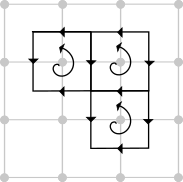
\includegraphics[scale=0.6]{figures/chapter4/schoenemann/schoenemann_cell_linel_orientation.png}
%}\hspace{0.5em}
%\subfloat[\label{ch4:fig:cell-complex-2}]{
%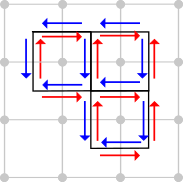
\includegraphics[scale=0.6]{figures/chapter4/schoenemann/schoenemann_oriented_edges.png}
%}\hspace{0.5em}
\subfloat[\label{ch4:fig:cell-complex-3}]{
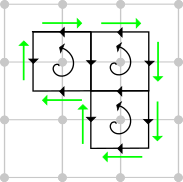
\includegraphics[scale=0.6]{figures/chapter4/schoenemann/valid_solution_0.png}
}\hspace{0.5em}
\subfloat[\label{ch4:fig:cell-complex-4}]{
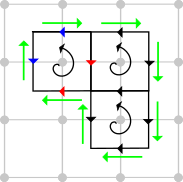
\includegraphics[scale=0.6]{figures/chapter4/schoenemann/valid_solution_1.png}
}\hspace{0.5em}
\subfloat[\label{ch4:fig:cell-complex-5}]{
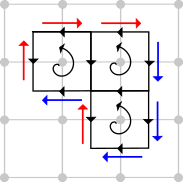
\includegraphics[scale=0.6]{figures/chapter4/schoenemann/valid_solution_2.png}
}
\caption{\textbf{Digital surface and consistency constraints.} In~\cref{ch4:fig:cell-complex-3}, a valid solution made of three cells and a sequence of eight linels. In~\cref{ch4:fig:cell-complex-4} the sum of linel-cell incidence equals to zero (blue are positively incident and red negatively incident). In~\cref{ch4:fig:cell-complex-5}, the sum of linel-edge incidence equals to zero.}
\label{ch4:fig:schoenemann-consistency-constraints}
\end{figure}

Let $n,m$ the number of cells and edges, respectively. We establish a convention on cells and linels orientation. We define the positive orientation of a cell as being counter-clockwise and the positive orientation of linels as being left (horizontal) and down (vertical), as indicated in the figure below. 

\begin{center}
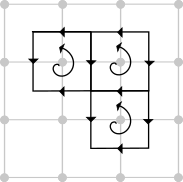
\includegraphics[scale=0.6]{figures/chapter4/schoenemann/schoenemann_cell_linel_orientation.png}
\end{center}

One binary variable is defined for each cell and two other binary variables are defined for each linel, one for each possible orientation the linel may assume. We refer to the variables associated to linels as edges. The variables are grouped in vector $\vec{x} \in \{0,1\}^{n+2m}$ and, hence, a solution is made of active cells and active edges. However, we have to make sure that solutions are consistent, i.e., a solution $\vec{x}$ must encode a digital surface. 

A digital surface is composed of a set of cells and a closed path (loop) of edges forming its boundary. To enforce digital surfaces, we define an incidence relation between linels and cells and between linels and edges. This relation is encoded by matrix $\vec{A} \in \{-1,0,1\}^{m\times(n+2m)}$ 

\begin{align*}
	\vec{A}_{i,j} &= \left\{ \begin{array}{rl}
		1,& \text{if positive incident}\\
		-1,& \text{if negative incident}\\
		0,& \text{otherwise}.		
	\end{array}\right.
\end{align*}

We say that a linel is positive incident to a cell if their orientations agree and negative incident if they disagree. Similarly, a linel is positive (negative) incident to an edge if they agree (disagree) in orientation. The space of solution is correctly restricted to digital surfaces by imposing

\begin{align*}
	\vec{A}\vec{x} &=0,
\end{align*}

i.e., the sum of incidences for each linel must equal to zero~(see~\cref{ch4:fig:schoenemann-consistency-constraints}). Finally, we set vector $\vec{w} \in \mathbb{R}^{n+2m}$ that is going to hold the data, length and squared curvature penalization terms. For example, data term coefficients are associated to cells variables while length and curvature terms are associated to edges. The complete formulation is written as

\begin{align*}
	\begin{array}{rl}
		\min_{\vec{x}} & \vec{w}^t\vec{x}\\
		\text{subject to} & \vec{A}\vec{x} = 0 \\
		& \vec{x} \in [0,1]^{n+2m},
	\end{array}
\end{align*}


where vector $\vec{x}$ was relaxed. The quality of the model naturally depends of the plane tessellation defined by the chosen cellular complex. A simple grid complex is not that interesting, as the discrete elastica can turn only on multiples of $\pi/2$. The authors present results for two different cellular complexes. They are equivalent to $8$-connectivity or $16$-connectivity in a graph-cut framework. 

The data term issue is handled by separating the roles of cells and edges. Cells variables holds data terms and edge variables hold curvature and length information. The refinement of the cellular complex is done via pixel subdivision, therefore, every cell lying in the interior of a pixel $p$ carries data term relative to pixel $p$. The consistency constraints guarantees well defined boundaries and the contour complexity issue is also covered. Finally, the model is extendable to different angular resolutions while keeping a digital setting, and a discrete elastica with an arbitrary sequence of interpolation points can be well approximated given a good choice of the cellular complex.

Some results are displayed in~\cref{ch4:fig:schoenemann-results}. However, the computation time is quite high and the segmentation present sharp angles even when employing a $16$-connectivity cellular complex.

\begin{figure}
\begin{minipage}{0.25\textwidth}
\center
\subfloat[\label{ch4:fig:schoenemann-connectivity-1}]{
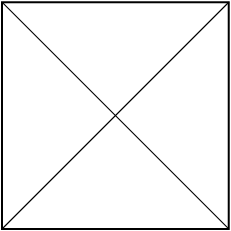
\includegraphics[scale=0.25]{figures/chapter4/schoenemann/neighborhood_system_8.png}
}

\subfloat[\label{ch4:fig:schoenemann-connectivity-2}]{
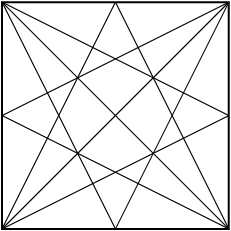
\includegraphics[scale=0.25]{figures/chapter4/schoenemann/neighborhood_system_16.png}
}
\end{minipage}%
\begin{minipage}{0.75\textwidth}
\center
\subfloat[\label{ch4:fig:schoenemann-results}]{
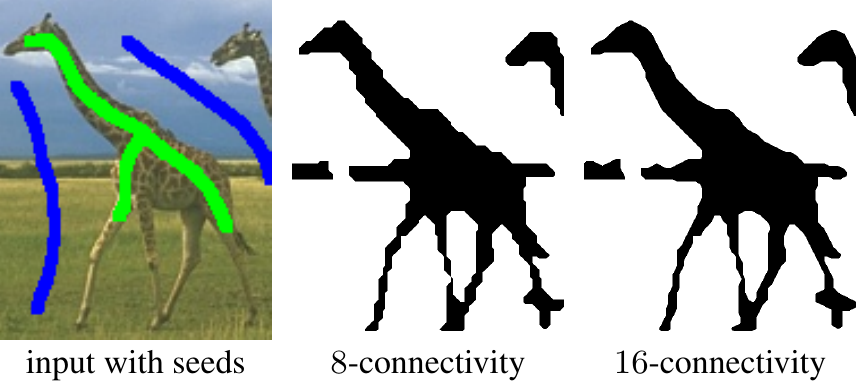
\includegraphics[scale=0.3]{figures/chapter4/schoenemann/schoenemann.png}
}
\end{minipage}%
\caption{\textbf{Linear programming model~\cite{schoenemann09linear}.} In the left, examples of the $8$ and $16$-connectivity cellular complexes. The authors implementation consists into subdivide a pixel. For example, the $8$-connectivity is implemented by rescaling the image twice its size and let the model unit being composed of $4$ pixels of the rescaled image. In the right, a result with different connectivities using a data term derived from given foreground (green) and background (blue) seeds. }
\end{figure}

\subsubsection{Unconstrained formulations}

The high number of variables and constraints explain the high running time of the linear programming approach. In~\cite{zehiry10fast}, the authors encode the squared curvature value in an unconstrained quadratic non-submodular PBF and propose a model for binary image segmentation.

Let $I$ be a digital image with $n$ pixels. We associate to each pixel the binary variable $\vec{x}_i$ indicating if the pixel belongs to foreground ($x_i=1$) or background ($x_i=0$). For a given segmentation $\vec{x}$, one can identify $90$ degrees turns in the segmentation contour by inspecting sequential pairs of vertices neighbors (given an order on the neighbors), as illustrated in figure~\cref{ch4:fig:elzehiry-turn-angles}. The turns can expressed as a $3$-clique potential, as shown in the table below

\begin{center}
\begin{tabular}{|c|c|c|c|}
\hline
$x_i$ & $x_j$ & $x_k$ & $w$ \\
\hline 
0 & 0 & 0 & 0 \\
0 & 0 & 1 & 0 \\
0 & 1 & 0 & 0 \\
0 & 1 & 1 & $w_{ijk}$ \\
1 & 0 & 0 & $w_{ijk}$ \\
1 & 0 & 1 & 0 \\
1 & 1 & 0 & 0 \\
1 & 1 & 1 & 0 \\
\hline 
\end{tabular}
\end{center}

\begin{figure}
\center
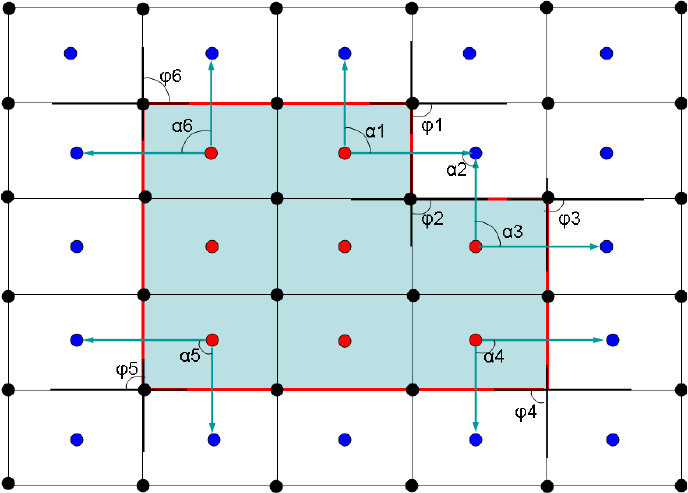
\includegraphics[scale=0.25]{figures/chapter4/elzehiry/turn-angles.png}
\caption{\textbf{Turn angles detection and triplets~\cite{zehiry10fast}.} Assuming that red pixels correspond to $1$-labeled variables and blue the $0$-labeled ones, angle variation is triggered by configurations $(x_i=1,x_j=0,x_k=0)$ and $(x_i=0,x_j=1,x_k=1)$, assuming that $x_i$ is the centered variable. }
\label{ch4:fig:elzehiry-turn-angles}
\end{figure}

The coefficients $w_{ijk}$ are defined accordingly with the Brucksteins discretization formula for the elastica, i.e.,

\begin{align*}
	w_{ijk} &= \frac{ \alpha_i ^2}{\min \{ |e_{ij}|,|e_{jk}| \} }.
\end{align*}

Remarkably, the $3$-clique potential can be decomposed in three $2$-cliques potentials 

\begin{align}
	E(x_i,x_j,x_k) &= w_{ij}(x_i-x_j)^2 + w_{ik}(x_i-x_k)^2 + w_{jk}(x_j-x_k)^2,
	\label{ch4:eq:elzehiry-pairwise}
\end{align}

where

\begin{align*}
	w_{ij} &= \frac{1}{2}w_{ijk} \\
	w_{ik} &= \frac{1}{2}w_{ijk} \\	
	w_{jk} &= -\frac{1}{2}w_{ijk}.
\end{align*}

~\cref{ch4:eq:elzehiry-pairwise} is a non-submodular PBF (the negative $w_jk$ coefficient creates a non-submodular term) and it is optimized using QPBO or one of its variations. The computation is much faster than the linear programming formulation and the model favors the connectivity principle, although the completion effect seems limited to very small portions~(see~\cref{ch4:fig:elzehiry-results}). A clear drawback is the limitation in the angle resolution, which tends to produce block artifacts. The authors argue that the model can be extended to any desired connectivity, but it is not clear how this is done.

\begin{figure}
\center
\begin{tabular}{ccc}
\subfloat[Original]{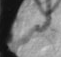
\includegraphics[scale=1.25]{figures/chapter4/elzehiry/vessel-1.png}} &
\subfloat[Data]{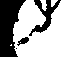
\includegraphics[scale=1.25]{figures/chapter4/elzehiry/vessel-2.png}} &
\subfloat[Data+Curvature]{\quad\quad 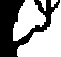
\includegraphics[scale=1.25]{figures/chapter4/elzehiry/vessel-3.png}\quad\quad} \\[1em]
\subfloat[Original]{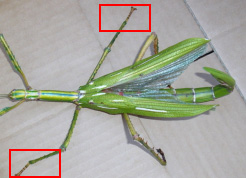
\includegraphics[scale=0.3]{figures/chapter4/elzehiry/insect-1.png}} &
\subfloat[Data]{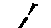
\includegraphics[scale=1.25]{figures/chapter4/elzehiry/insect-2.png}} &
\subfloat[Data+Curvature]{\quad\quad 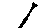
\includegraphics[scale=1.25]{figures/chapter4/elzehiry/insect-3.png}\quad\quad}
\end{tabular}
\caption{\textbf{Results for the grid graph model~\cite{zehiry10fast}.} The original image is displayed in the left; segmentation using only data in the middle; and the segmentation using squared curvature regularization in the right. Connectivity is encouraged, but to a very limited extension.}
\label{ch4:fig:elzehiry-results}
\end{figure}

In~\cite{nieuwenhuis14efficient} is presented an alternative formulation that is extendable to any desirable angle resolution. The idea is in fact quite similar to the one in~\cite{zehiry10fast} in the sense that curvature is measured by counting the number of configurations $(0,1,0)$ and $(1,0,1)$ of triplets of vertices. Intuitively, as illustrated in~\cref{ch4:fig:nieuweinhuis-triplets-1}, the curvature is higher at regions in which these configurations are more frequent. The authors prove the following theorem

\begin{figure}
\center
\subfloat[\label{ch4:fig:nieuweinhuis-triplets-1}]{
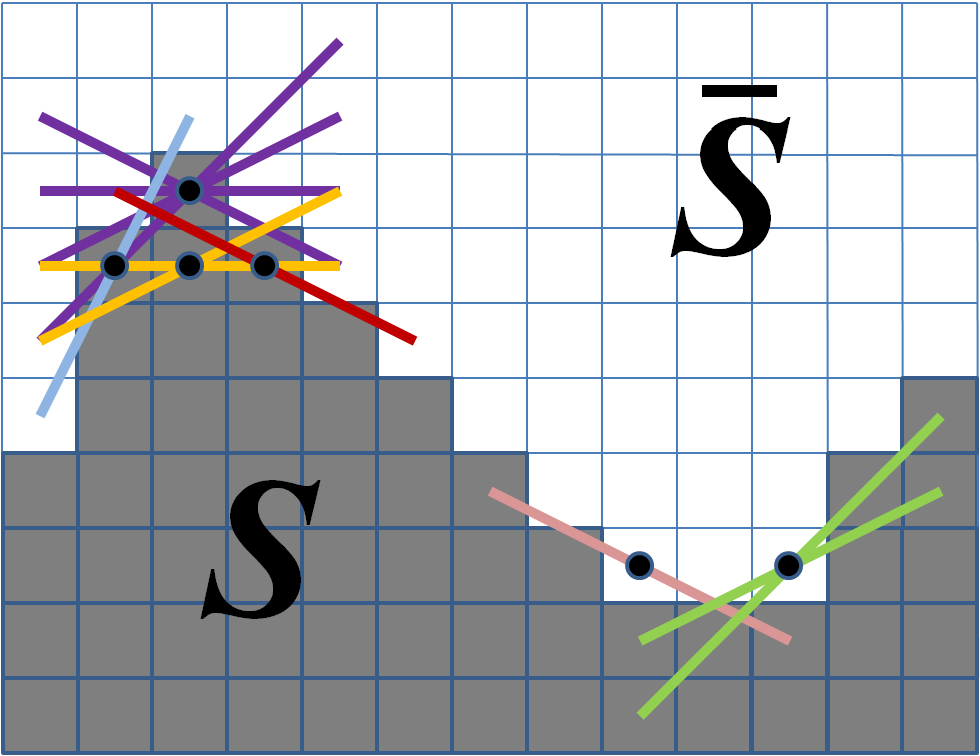
\includegraphics[scale=0.1]{figures/chapter4/nieuweinhuis/triplets.png}
}
\subfloat[\label{ch4:fig:nieuweinhuis-triplets-2}]{
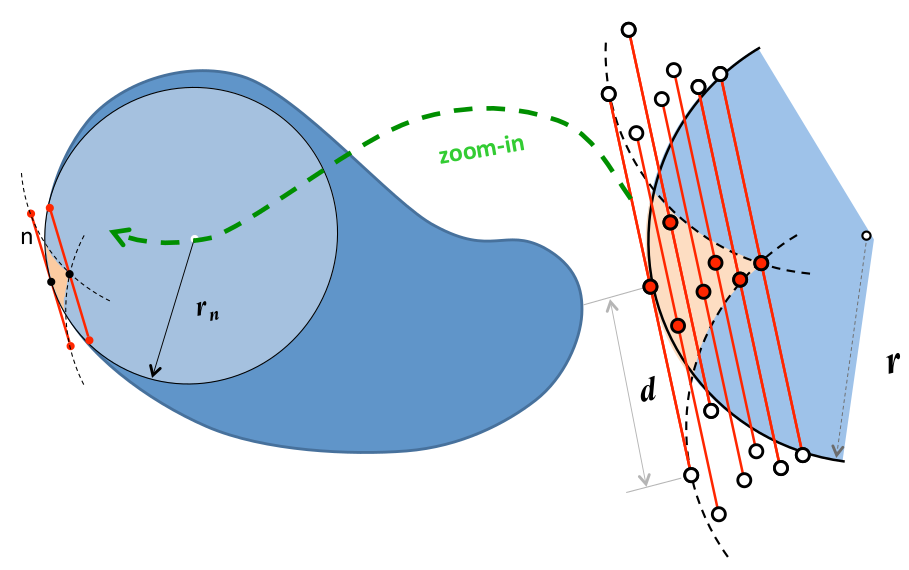
\includegraphics[scale=0.25]{figures/chapter4/nieuweinhuis/nieuwenhuis_brown_area.png}
}
\caption{\textbf{Triplets configurations and integral geometry~\cite{nieuwenhuis14efficient}.} In~\cref{ch4:fig:nieuweinhuis-triplets-1} we intuitively notice that curvature is higher where triplets configurations $(0,1,0)$ and $(1,0,1)$ are perceived. In~\cref{ch4:fig:nieuweinhuis-triplets-2}, an illustration of~\cref{ch4:thm:nieuweinhuis}. }
\label{ch4:fig:nieuweinhuis-triplets}
\end{figure}

\begin{theorem}{\cite{nieuwenhuis14efficient}}\label{ch4:thm:nieuweinhuis}
Let contour point $n$ have tangent orientation $t$ and osculating ball $B_r$ of radius $r=1/|k|$. Then, the set of all points $p \in B_r$ such that $\norm{p-n} \leq r$ and $(p \pm d \cdot t) \notin B_r$ for given distance $d < r$ has area 

\begin{align*}
	A(\kappa,d) &= \frac{|\kappa|d^3}{4} + O(d^4).
\end{align*}

\end{theorem}

Notice that the theorem is valid for cliques aligned with the tangent at the point of curvature computation. The set of available cliques orientations is defined according to the chosen neighborhood. The neighborhood system of size $(2d+1) \times (2d+1)$ for pixel $p$ is similar to a digital circle of radius $d$ centered at $p$ (although not the same), in the sense that the neighbors of $p$ are chosen in order to have approximately the same distance $d$ from $p$~(see~\cref{ch4:fig:nieuweinhuis-neighborhood}). The larger the value of $d$, the greater the chances to have a triplet orientation that matches the tangents along the object contour.

\begin{figure}
\center
\subfloat[$d=2$]{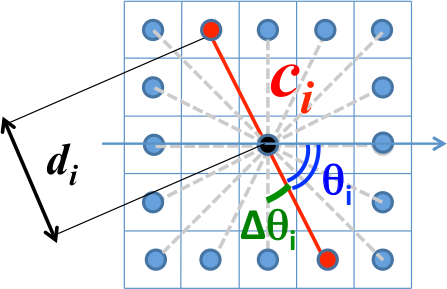
\includegraphics[scale=0.3]{figures/chapter4/nieuweinhuis/nieuwenhuis_neighborhood_1.png}
}\hspace{2em}
\subfloat[$d=3$]{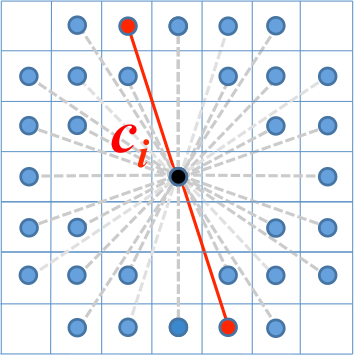
\includegraphics[scale=0.3]{figures/chapter4/nieuweinhuis/nieuwenhuis_neighborhood_2.png}
}
\caption{\textbf{Neighborhood system~\cite{nieuwenhuis14efficient}.} The higher the value of $d$, the higher is the angle resolution.}
\label{ch4:fig:nieuweinhuis-neighborhood}
\end{figure}

Let $d$ be the chosen neighborhood system and $c_i$ the corresponding triplets in this neighborhood. Moreover, assume that the triplets are ordered with respect the angle made with the horizontal axis. Let $\Delta \theta_i$ be the angle difference between two consecutive triplets and $i(p)$ the triplet index with the closest orientation to the tangent at $p$. The integral squared curvature is approximated by 

\begin{align*}
	\int_{C}{\kappa ^2 ds} &\approx \sum_{p}{ |\kappa_{p}|\Delta \theta_{i(p)}} \\
	&= \sum_{p} \frac{4\Delta \theta _{i(p)}}{d^3_{i(p)}} \cdot A(\kappa_p,d_{i(p)}) \\
	&\approx \sum_{i}\sum_{p} \frac{4\Delta \theta _i}{d^3_i} \cdot \delta(c_i(p)),
\end{align*}

where the function $\delta$ is one for triplets configurations $(0,1,0)$ or $(1,0,1)$ and zero otherwise. The function delta can be expressed as

\begin{align*}
	\delta(x_a,x_b,x_c) &= x_i(1-x_j)x_k + (1-x_i)x_j(1-x_k) \\
	&= x_j + x_ix_k - x_ix_j - x_jx_k.
\end{align*}

The resulting energy is non-submodular (the positive term in the $\delta$ function is non-submodular) and is solved using the LSA-TR method~\cite{gorelick14local}, reported to produce better results than QPBO for some non-submodular instances. Some results for inpainting and segmentation are shown in~\cref{ch4:fig:nieuweinhuis-results}. The model is unconstrained, extendable to arbitrary angle resolution and can be easily modified to include data and length terms. 
X
Although an argument is provided to justify the curvature approximation, it is difficult to do a multigrid analysis, i.e., to analyse its convergence over different resolutions. The experiments provided by the authors are limited to the computation of the elastica along a disk, and we are not sure about the behaviour of such estimator in shapes of more complex geometry. The fundamental goal of this thesis is to investigate imaging models using geometric penalization estimated by proven multigrid convergent estimators. In the next chapter we explore the multigrid convergence property and some other concepts of digital geometry.

\begin{figure}
\center
\begin{tabular}{ccc}
\subfloat[Original.]{
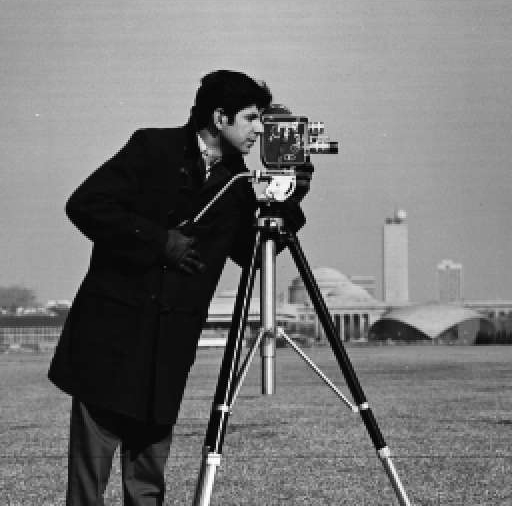
\includegraphics[scale=0.25]{figures/chapter4/nieuweinhuis/camera-man-1.png}} &
\subfloat[Binary segmentation.]{
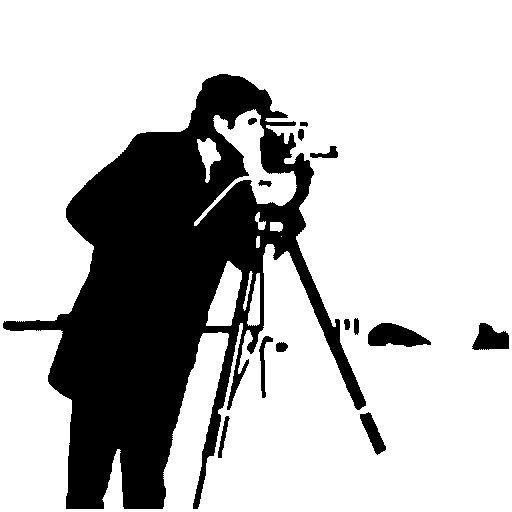
\includegraphics[scale=0.25]{figures/chapter4/nieuweinhuis/camera-man-2.png}} &\\
\subfloat[Original and inpainting masks.]{
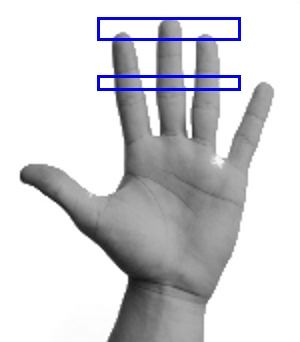
\includegraphics[scale=0.25]{figures/chapter4/nieuweinhuis/hand-1.png}} &
\subfloat[Inpainting with length regularization.]{\quad\quad
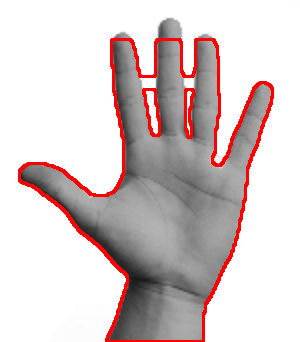
\includegraphics[scale=0.25]{figures/chapter4/nieuweinhuis/hand-2.png}\quad\quad} &
\subfloat[Inpainting with curvature regularization.]{
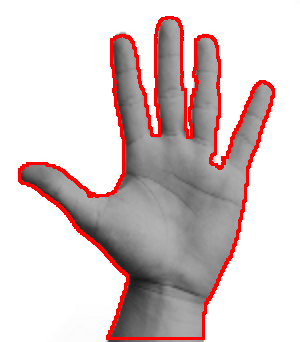
\includegraphics[scale=0.25]{figures/chapter4/nieuweinhuis/hand-3.png}}
\end{tabular}
\caption{\textbf{Segmentation and inpainting results~\cite{nieuwenhuis14efficient}.} The connectivity principle is perfectly illustrated in the inpainting problem but one would expect a completion of the rightmost bar of the camera tripod. }
\label{ch4:fig:nieuweinhuis-results}
\end{figure}



%
%\section{Chapter notes}
%
%the derived the following 
%
% to solve tasks as basic as edge detection. The curvature appeared in the context of diffusion methods, for example, consider the Perona-Malik edge detector. 
%
%Earlier appearances of curvature in image processing model dates back to the use
%
%The curvature appear in earlier models of image processing based on anisotropic diffusions. Take for example the edge detection task. The 
%
%The curvature is present in models of image processing even for the lowest-level tasks as edge detection. 
%
%Earlier models of image processing diffusion based 
%
%appears very often in models of image processing. 
%
%The curvature is presented in early models of image processing, some of them presented in~\cref{chapter:variational-methods-in-image-processing} as the Geometric Active Contour for image segmentation and Total Variation for image denoising.
%
%
%%\sketch{
%%\begin{enumerate}
%%	\item{Motivation}
%%	\item{Wave equation (Diprima)ter}
%%	\begin{itemize}
%%		\item{Curvature properties}
%%	\end{itemize}
%%	\begin{itemize}
%%		\item{Constraint optimization models}
%%		\item{Combinatorial optimization models}		
%%		\item{Continuous models}
%%	\end{itemize}
%%	
%%\end{enumerate}
%%}
%
%Por que nao usar diferencas finitas pra modelar curvatura ao quadrado?
%
%Por que nao usar elementos finitos para modelar curvatura ao quadrado?
%
%Qual o problema com a resolucao numerica de equacoes diferenciais de ordem alta?
%
%Inpainting de objetos com textura x objetos sem textura (PDE tende a suavizar em excesso e por isso nao seria apropriado para texturas. Mas o TV metodo eh capaz preservar em parte as discontinuidades. Bem, talvez em uma imagem super texturizada mesmo TV nao seja suficiente)
%
%Em PDEs de segunda ordem o passo do tempo artificial pode ser maior do que aquele de uma
%equacao de terceira ordem sem ter consequencias de divergencia.
%
%Mean curvature motion
%
%Derivacoes de curvatura. Curvatura de funcao implicita e a curvatura de level sets.
%
%Elastica. Derivacao do resultado da Free Elastica. Balloon and shrinking forces. Perimeter minimization is the energy being minimized by the mean curvature flow; the squared curvature term, on the other hand, contributes to grow the shape.
%
%
%Cubic splines and Elastica. Non linear splines study by Birkhof at General Motors.
